\documentclass[a4paper]{IEEEtran}

% Ein paar hilfreiche Pakete
\usepackage{german}
\usepackage[utf8]{inputenc}
\usepackage{graphicx} 
\usepackage{amsmath} 
\usepackage{amssymb}  
\usepackage{mathtools}
\mathtoolsset{showonlyrefs}
\usepackage{subfigure}
\usepackage{flushend}
\usepackage{url}

% Ein paar am ISAS übliche Formelzeichen
\def\rv#1{{\mathbf #1}} %Random Variable
\def\vec#1{\underline{#1}} %Vector
\def\rvv#1{{\vec{\rv{#1}}}} %Random Vector
\def\mat#1{{\mathbf #1}} %Matrix
\def\Var{\mathrm{Var}} %Variance
\def\E{\mathrm{E}} %Expectation
\def\Cov{\mathrm{Cov}} %Covariance
\def\IN{\mathrm{I\hspace{-2pt}N}} %Natural Numbers
\def\IR{\mathrm{I\hspace{-2pt}R}} %Real Numbers 

% correct bad hyphenation here
\hyphenation{op-tical net-works semi-conduc-tor}


\begin{document}
\title{Markov-Entscheidungsprozesse für die Roboterpfadplanung}

\author{Matthias~Holoch,~\IEEEmembership{E-Mail: matthias.holoch@student.kit.edu}}% <-this % stops a space




% The paper headers
\markboth{Proseminar WS 12/13: Anthropomatik: Von der Theorie zur Anwendung}%
{Proseminar WS 12/13: Anthropomatik: Von der Theorie zur Anwendung}



% make the title area
\maketitle


\begin{abstract}
Markov-Entscheidungsprozesse sind ein in vielen Gebieten beliebter Weg, um Entscheidungsprobleme in Umgebungen mit Unsicherheiten zu modellieren. Eines der Gebiete, in denen Unsicherheit eine große Rolle spielt, ist die Pfadplanung von autonomen Robotern. Diese Ausarbeitung beschäftigt sich in erster Linie mit dem vollständig beobachtbaren Markov-Entscheidungsprozess in Bezug auf die Roboterpfadplanung.
\end{abstract}


\section{Einleitung}
Der vollständig beobachtbare Markov-Entscheidungsprozess (englisch: \emph{completely observable Markov decision process}, kurz coMDP, im Folgenden als MDP bezeichnet) ist ein mathematisches Modell zur Modellierung von Entscheidungsproblemen. Der MDP wird verwendet, um Systeme, bei denen Aktionen nicht deterministische Folgen haben können zu modellieren und dann aus diesem Modell eine Strategie, also eine Aktion für jeden Zustand, zu errechnen.

In fast allen Bereichen können Unsicherheiten auftreten, was dazu führt, dass der Einbezug von Unsicherheiten in das Modell in vielen Bereichen äußerst interessant ist. Da es für ein reales Entscheidungsproblem nie möglich ist, dessen Eigenschaften vollständig und exakt in ein Modell zu überführen wird sich so ein Modell immer in gewissem Maße von der Wirklichkeit unterscheiden. Dadurch entsteht schon allein wegen des modellbasierten Vorgehens ein gewisses Maß an Unsicherheit.

In \cite{cassandra1998survey} werden eine ganze Reihe von verschiedenen Anwendungsbereichen für Markov-Entscheidungsprozesse beschrieben. So verursachen im Bereich der autonomen Roboter äußere Störungen, wie zum Beispiel Schlupf, unterschiedliche Beschaffenheit des Bodens oder Fehlerrauschen an den Sensoren zusätzliche Unsicherheiten.

In der Verhaltensökologie kann unter der Annahme, dass sich Organismen immer optimal in Bezug auf ihr internes Modell der Welt verhalten, mit Hilfe von Markov-Entscheidungsprozessen so ein Modell nachgebaut werden. Daraufhin werden die aus dem nachgebauten Modell berechneten Verhaltensweisen mit den tatsächlichen Verhaltensweisen des Organismus verglichen und bei Abweichungen das nachgebaute Modell verbessert. Dieses Vorgehen führt zu einem besseren Verständnis des Verhaltens des Organismus.

Es gibt auch eine Vielzahl von nicht-wissenschaftlichen Anwendungsbereichen. So erschließt sich beispielsweise im Bereich der medizinischen Diagnose dem Arzt niemals der genaue Zustand des Patienten. Viel mehr stehen ihm ein beschränktes Maß an Aktionen wie zum Beispiel Labortests oder das Verabreichen von Medikamenten zur Verfügung. Daraufhin kann der Arzt verschiedene Reaktionen beobachten, die mit einem gewissen Maß an Unsicherheit auf seinen Zustand schließen lassen und muss sich an Hand derer für eine weitere Behandlung entscheiden. 

Das Konzept der MDPs wird im Folgenden anhand eines Beispiel aus dem Bereich der autonomen Roboter veranschaulicht. Das angeführte Beispiel basiert auf \cite{thrun2005probabilistic}.


\section{Planung unter Unsicherheit}
\label{sec:planning}
\begin{figure}[ht]
	\centering
	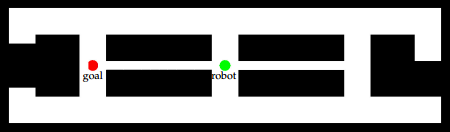
\includegraphics[scale=0.72]{images/autnmRobot_basicSituation.png}
	\caption{Eine beispielhafte Umgebung mit Roboter und Ziel. Der Roboter befindet sich mittig mit der Aufgabe sich zu dem Zielpunkt im linken Bereich der Umgebung zu bewegen (aus \cite{thrun2005probabilistic}).}
	\label{fig:autnmRob_bSit}
\end{figure}

Wie in Abbildung \ref{fig:autnmRob_bSit} dargestellt betrachten wir im Folgenden einen autonomen Roboter der sich im Zentrum einer nahezu symmetrischen Umgebung befindet. Im linken Bereich der Umgebung befindet sich ein Ziel. Die Aufgabe des Roboters ist es, das Ziel zuverlässig und möglichst schnell zu erreichen. Es existieren mehrere Pfade die den Roboter an das Ziel bringen. Einen kurzen Pfad, der durch den engen Korridor führt und zwei längere, breitere Pfade außen herum.

In der klassischen Planung für Roboter existiert keine Unsicherheit. Es wird angenommen der Roboter kenne seine Position und die des Zielpunktes exakt. Zusätzlich haben ausgeführte Aktionen genau vorhersehbare Effekte. In dieser Situation würde vor Aktionsausführung die Vorberechnung einer einzelnen Abfolge von Aktionen, die den Roboter sicher und möglichst schnell an das Ziel bringt, ein leichtes sein. Der Einbezug von Sensordaten während der Aktionsausführung wäre unnötig, da der Roboter absolut fehlerfrei funktioniert.

\begin{figure}[ht]
	\centering
	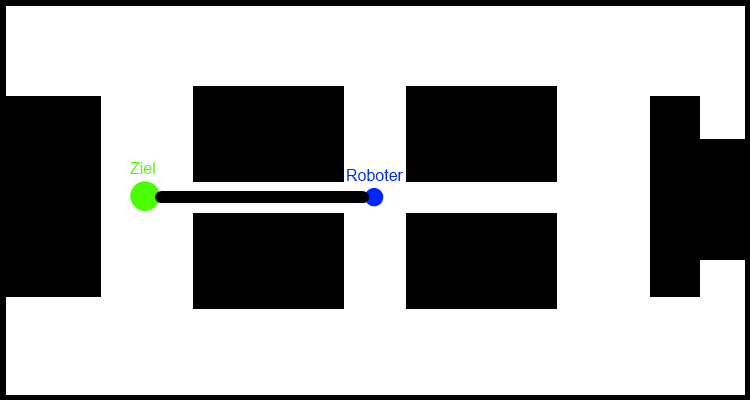
\includegraphics[scale=0.72]{images/autnmRobot_directPath.png}
	\caption{Ohne die Anwesenheit von Fehlern in der Bewegung des Roboters ist der kürzere, enge Pfad dem längeren, breiten Pfad klar überlegen (aus \cite{thrun2005probabilistic}).}
	\label{fig:autnmRob_dirPath}
\end{figure}

Abbildung \ref{fig:autnmRob_dirPath} zeigt eine solche vorberechnete Aktionsfolge. Da bisher angenommen wurde, dass der Roboter absolut fehlerfrei funktioniert ist der kürzere, enge Pfad jedem der längeren, breiten Pfade vorzuziehen.

In der Praxis funktionieren solche einfachen Aktionsfolgen meist aus mehreren Gründen nicht richtig: Ein Roboter, der blind einem engen Korridor folgt läuft Gefahr mit den Wänden zu kollidieren. Außerdem ist es sehr wahrscheinlich, dass der Roboter auf Grund des während der Aktionsausführung akkumulierten Fehlers das Ziel verfehlt.

Daher werden in der Praxis häufig Planungsalgorithmen dieser Art mit einem sensorbasierten Kontrollmodul kombiniert. Dieses Kontrollmodul verwendet die Sensordaten des Roboters um Fehler, die bei der Aktionsausführung auftreten, zu erkennen, und den Roboter immer wieder auf den geplanten Kurs zurück zu führen. Insbesondere bei einem Fall wie dem engen Korridor in unserem Beispiel muss so eine Korrektur besonders häufig stattfinden, um eine Kollision mit der Wand des Korridors zu vermeiden. Dadurch wird eine größere Zahl an Messungen benötigt, die eine signifikante Verringerung der Fortbewegungsgeschwindigkeit des Roboters mit sich bringen, die von dem klassischen Planungsalgorithmus nicht berücksichtigt wird. 

\begin{figure}[ht]
	\centering
	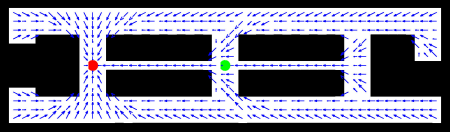
\includegraphics[scale=0.72]{images/autnmRobot_detActionMDP.png}
	\caption{Darstellung einer Strategie bei \emph{nicht} probabilistischen Effekten bei der Aktionsausführung. Hier ist der kurze Pfad klar überlegen (aus \cite{thrun2005probabilistic}).}
	\label{autnmRobot_detA}
\end{figure}
\begin{figure}
	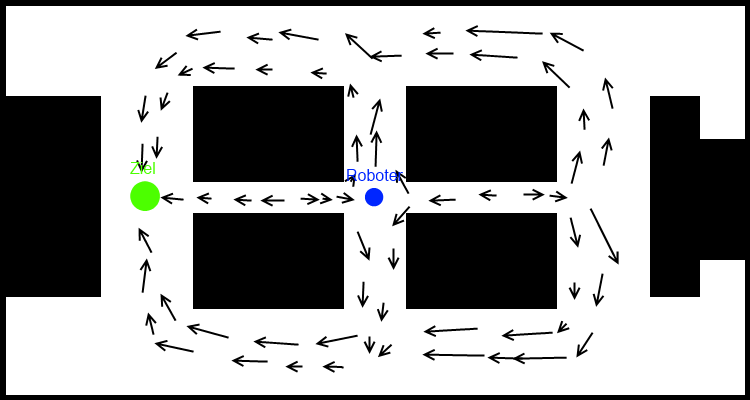
\includegraphics[scale=0.72]{images/autnmRobot_ndetActionMDP.png}
	\caption{Darstellung einer Strategie bei probabilistischen Effekten bei der Aktionsausführung. Hier wird der längere Pfad bevorzugt (aus \cite{thrun2005probabilistic}).}
	\label{autnmRobot_ndetA}
\end{figure}

Als Konsequenz muss eine präzisere Herangehensweise nicht lediglich eine einzelne Aktionsabfolge vorberechnen, sondern mehrere Aktionen für eine Vielfalt an Situationen, in die der Roboter auf Grund seiner unvorhersehbaren, fehlerbehafteten Aktionsausführung geraten könnte.

Um eine solche Aktionsfolgen vorberechnen zu können benötigen wir ein Modell, welches stochastische Effekte in der Aktionsausführung berücksichtigt. Ein solches Modell ist der MDP. Eine aus einem MDP berechnete Strategie gibt für jeden Zustand der Umgebung, hier der Ort, an dem sich der Roboter befindet, eine bestmögliche Aktion an. In diesem Beispiel ist eine solche Aktion eine Bewegung in eine bestimmte Richtung. Egal ob bei der Bewegung Fehler auftreten oder nicht, der Roboter kann danach mit seinen Sensoren seinen Ort erneut feststellen und findet in der vorberechneten Strategie eine nächste optimale Aktion.

Abbildung \ref{autnmRobot_detA} zeigt eine solche Vorberechnung für einen Roboter mit fehlerfreier Aktionsausführung. Hier wählt die Strategie bevorzugt den Weg durch den engen, kurzen Korridor. Bei der Ausführung würde diese Vorberechnung zu dem selben Ergebnis führen wie die vorberechnete Aktionsfolge in Abbildung \ref{fig:autnmRob_dirPath}. In Abbildung \ref{autnmRobot_ndetA} ist eine Vorberechnung für einen Roboter mit fehlerbehafteter Aktionsausführung dargestellt. Hier wird hingegen einer der längeren, breiten Pfade bevorzugt.

Allerdings setzt der MDP voraus, dass der Agent, in unserem Beispiel der Roboter, den Zustand der Umgebung zu jedem Zeitpunkt exakt erkennen kann. Wir müssten also annehmen, dass die Sensoren des Roboters perfekt funktionieren.

In der Praxis ist natürlich auch diese Annahme nicht haltbar. Jedes Sensormodul hat mehr oder weniger stark ausgeprägtes Fehlerrauschen. Bei den meisten Anwendungen, wie auch bei unserem Beispiel, kommt sogar noch ein weiteres Problem hinzu: Falls der Roboter lediglich über Distanz- oder Winkelsensoren verfügt, dann ist es ihm auf Grund der Symmetrie der Beispielumgebung nicht möglich festzustellen, wie er orientiert ist und damit in welcher Richtung das Ziel liegt.

Ein solches Modell, der teilweise beobachtbare Markov-Entscheidungsprozess (englisch: \emph{partially observable Markov decision process}, kurz: POMDP), wird in Kapitel \ref{sec:pomdp} dieser Ausarbeitung kurz angerissen.

\section{MDP}
\begin{figure}[ht]
	\centering
	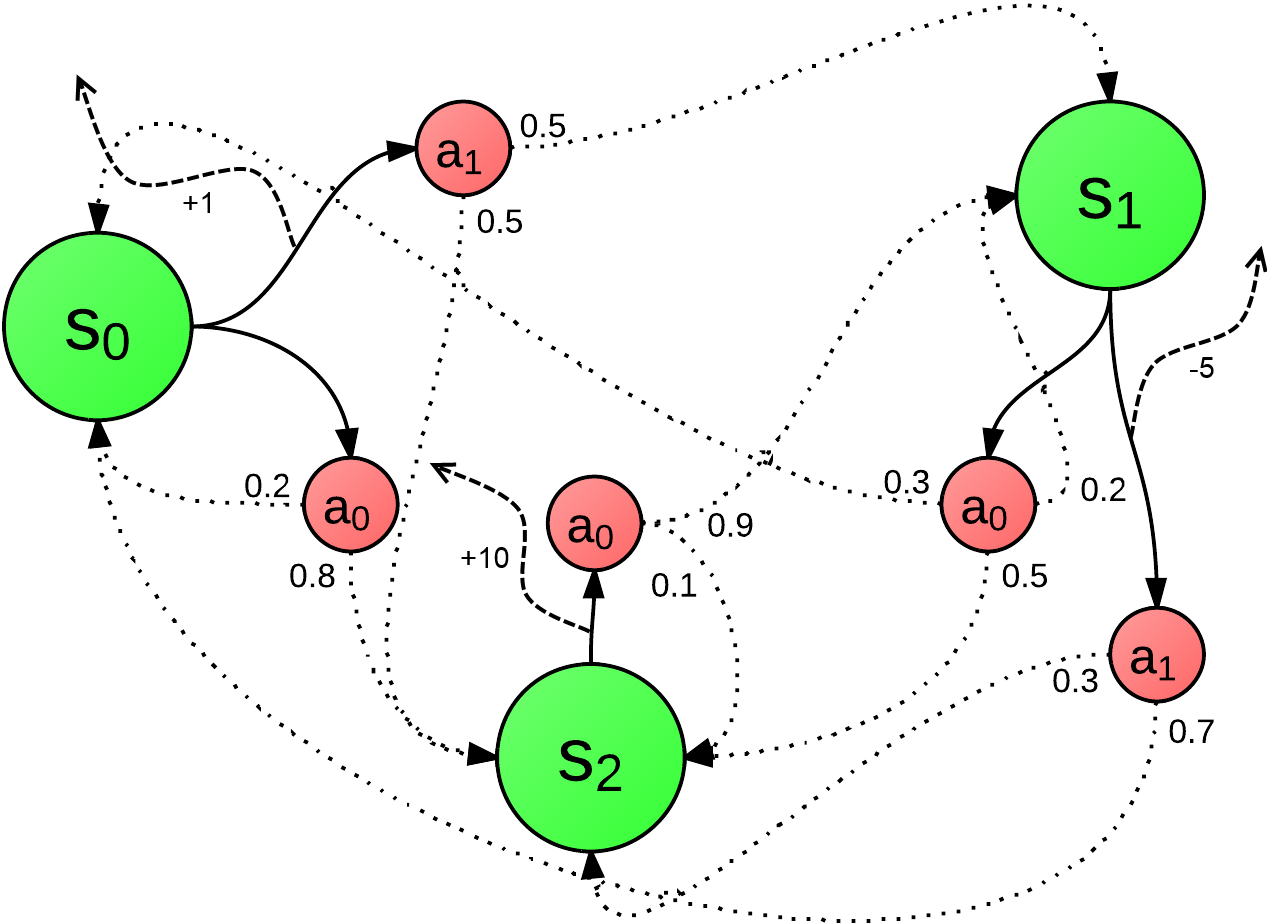
\includegraphics[scale=0.60]{images/MDP_example.png}
	\caption{Beispiel eines simplen MDP mit drei Zuständen $s_1, s_2, s_3$ und zwei Aktionen $a_0$ und $a_1$ dargestellt als Graph.}
	\label{fig:MDP_example} %TODO Dieses Bild ist durch die Änderung der Definition nicht mehr passend. Am besten selbst ein Bild machen.
\end{figure}
Nach \cite{cassandra1995acting} ist ein MDP definiert als ein 4-Tupel
\begin{equation}
	(S, A, T, R) \ .
\end{equation}
Es gibt die folgenden grundlegenden Komponenten:
\begin{itemize}
	\item Die diskrete, endliche Zustandsmenge $S$ enthält alle möglichen Zustände, in denen sich das System befinden kann. Der Agent kann jederzeit exakt feststellen, in welchem Zustand sich das System befindet.
	\item Die endliche Menge der Aktionen $A$.
	\item $T$ ist das Zustandsübergangsmodell des Systems. Es ist eine Funktion, welche Elemente aus $S \times A$ auf eine diskrete Wahrscheinlichkeitsverteilung über $S$ abbildet. Der Übergang
	\begin{equation}
		T(s, a, s')
	\end{equation}
	drückt die Wahrscheinlichkeit aus, dass sich die Umgebung nach Wählen der Aktion $a$ in Zustand $s$ im Zustand $s'$ befindet.
	\item Die Funktion
	\begin{equation}
		r: S \times A \rightarrow \IR
		\label{eq:payoff}
	\end{equation}
	drückt die Güte (englisch: \emph{payoff}), für den Agenten in Abhängigkeit von der gewählten Aktion in einem Zustand aus. Für das hier behandelte Anwendungsgebiet werden Kosten werden als negative Zahlen und Belohnungen als positive Zahlen dargestellt.
\end{itemize}
In Abbildung \ref{fig:MDP_example} ist ein MDP mit drei Zuständen $s_1, s_2, s_3$ und zwei Aktionen $a_0$ und $a_1$ als Graph dargestellt. Für jeden Zustand $s \in S$ gibt es eine Teilmenge $A_s \subseteq A$ von Aktionen von denen ausgehende Kante die Wahrscheinlichkeit des Übergangs in den entsprechenden Folgezustand als Kantengewicht darstellen. Die gestrichelten Pfeile symbolisieren die Güte (siehe \ref{eq:payoff}) bestimmter Aktionen in bestimmten Zuständen.

In mancher Literatur finden sich auch leicht anders geartete Definitionen. In \cite{russell1995artificial} ist beispielsweise die Gütefunktion eine Funktion, die lediglich von dem Zustand abhängt und es gibt eine Teilmenge $S_{terminal} \subseteq S$ der Zustandsmenge die als Terminalzustände bezeichnet werden. Sobald sich der Agent in einem Terminalzustand befindet kann er keine Aktionen mehr durchführen. Dadurch kann die Modellierungen bestimmter Umgebungen vereinfacht werden, verändert das Problem nur unwesentlich.


\section{Strategien aus dem MDP}
\subsection{Motivation}
Nun ist ein Modell definiert, welches stochastische Effekte in der Aktionsausführung berücksichtigt. Damit der Roboter aus unserem Beispiel tatsächlich etwas mit dieser Art der Modellierung anfangen kann, muss ein Weg gefunden werden, um aus dem Modell mehrere verschiedene Aktionsfolgen vor zu berechnen, denn eine einzelne festgelegte Sequenz an Aktionen funktioniert aus den in Kapitel \ref{sec:planning} angeführten Gründen selten gut. Stattdessen muss eine Strategie (englisch: \emph{policy}) für jeden möglichen Systemzustand $s \in S$ festlegen, was zu tun ist. Eine solche Strategie ist definiert als
\begin{equation}
	\pi:S \rightarrow A
	\label{eq:policy}
\end{equation}
und $\pi(s)$ ist die von der Strategie $\pi$ vorgegebene Aktion im Zustand $s$. Hat der Roboter eine solche Strategie ist immer klar, was er als nächstes zu tun hat - unabhängig davon, was bei der Aktionsausführung tatsächlich geschieht.

\subsection{Optimale Strategie}
Ob eine Strategie optimale ist unterscheidet sich von Anwendung zu Anwendung. Bevor eine optimale Strategie vor berechnet werden kann, muss zu erst definiert werden, was optimal tatsächlich bedeutet. In diesem Kontext ist der Planungshorizont (englisch: \emph{planning horizon}) ein wichtiges Konzept. In manchen Fällen kann es reichen eine Strategie so zu wählen, dass die unmittelbare Belohnung maximiert wird. In den meisten Fällen zahlen sich Aktionen aber nicht sofort aus. In unserem Beispiel wäre eine Gütefunktion
\begin{equation}
	r(s,a) = \left\{ \begin{array}{rl}
		+100 &\mbox{ falls $a$ in das Ziel führt} \\
		-1 &\mbox{ sonst}
       \end{array} \right.
\end{equation}
denkbar. Hier wird deutlich erkennbar, dass die Belohnung erst nach vielen Aktionen eintritt. Daher kann eine Strategie, die lediglich die unmittelbare Belohnung maximiert hier kein optimales Ergebnis liefern: Jede Aktion, egal ob sie in Richtung des Ziels oder vom Ziel weg führt hat die Kosten -1 und wären somit für eine solche Strategie gleichwertig.
Stattdessen setzt man sich häufig zum Ziel die Summe der zukünftigen Belohnungen zu maximieren.

Die folgenden Ausführungen basieren auf \cite{russell1995artificial}. Zunächst wird der Nutzen (englisch: \emph{utility}) einer Aktionsfolge 
\begin{equation}
	U([(s_0, a_0), (s_1, a_1), ..., (s_n, a_n)])
\end{equation}
definiert. Ist unser Planungshorizont endlich, dann gibt es einen Zeitpunkt $n \in N$ nach dem Aktionen des Agenten nichts mehr Wert sind. Demnach ist 
\begin{equation}
	\begin{split}
		U([ (s_0, a_0), (s_1, a_1), ..., (s_n, a_n)]) \\
		= U([ (s_0, a_0), (s_1, a_1), ..., (s_{n+k}, a_{n+k})]),\\
		\forall k \in \IN \ .
	\end{split}
\end{equation}
Dadurch kann es vorkommen, dass beispielsweise ein Zielpunkt mit besonders hoher Belohnung zu einem bestimmten Zeitpunkt von manchen Zuständen aus nicht mehr erreicht werden kann und daher die optimale Aktion in einem diesen Zuständen eine andere ist, als wäre der Agent zu einem früheren Zeitpunkt in einem dieser Zustände gewesen. Daher kommt der Effekt, dass sich bei einem endlichen Planungshorizont die optimale Aktion in demselben Zustand über die Zeit verändern kann. Die optimale Strategie für einen endlichen Planungshorizont ist also \emph{nicht stationär}.

Diese Problematik existiert nicht, wenn ein unendlichen Planungshorizont angenommen wird. Dann gibt es keinen Grund zu verschiedenen Zeitpunkten eine andere Aktion in demselben Zustand zu wählen.

Es gibt mehrere Möglichkeiten einer Aktionsfolge einen Nutzen zuzuweisen:
\begin{enumerate}
	\item \textbf{Additive Güte:} (englisch: \emph{additive rewards})
		\begin{equation}
			U([ (s_0, a_0), (s_1, a_1), ..., (s_n, a_n)]) = \sum\limits_{t=1}^n r(s_t, a_t)\ .
		\end{equation}
		Die additive Güte funktioniert nur dann gut, wenn der Planungshorizont endlich ist. Bei einem unendlichen Planungshorizont ($n \rightarrow \infty$) divergiert die Wertefunktion und zwei Aktionsfolgen können nicht mehr unterschieden werden. Als anschauliches Beispiel kann man sich zwei Arbeitsplätze vorstellen, von denen der eine 1 Geldeinheit pro Stunde und der andere 10 Geldeinheiten pro Stunde einbringt. Bei unendlichem Planungshorizont bringen beide Jobs unendlich viel Geldeinheiten ein und sind dadurch für die Strategie gleichwertig.
	\item \textbf{Reduzierte Güte:} (englisch: \emph{discounted rewards})
		\begin{equation}
			\begin{split}
				U([ (s_0, a_0), (s_1, a_1), ..., (s_n, a_n)]) = \sum\limits_{t=1}^n \gamma^t r(s_t, a_t),\\
				\text{mit }\gamma \in [0,1]\ .
			\end{split}
		\end{equation}
		Der Reduzierungsfaktor $\gamma$ (englisch: \emph{discount factor}) drückt aus, wie wichtig die zeitliche Nähe der Belohnung ist. Für $\gamma=1$ lässt sich mit der reduzierten Güte auch das additive Modell darstellen. Die additive Güte ist also ein Spezialfall der reduzierten Güte. Nach \cite{thrun2005probabilistic} gilt für $\gamma < 1$ und bei beschränkter Güte 
		\begin{equation}
			\exists r_{max} \in \IR\ \forall s \in S\ \forall a \in A: |r(s,a)| < r_{max} \ ,
		\end{equation}
		dass die Wertefunktion auch bei unendlichem Planungshorizont konvergiert. Der Nutzen einer Aktionsfolge lässt sich dann abschätzen mit  
		\begin{equation}
			\sum\limits_{t=1}^n \gamma^t r(s_t, a_t) \leq \sum\limits_{t=1}^n \gamma^t r_{max} = \frac{r_{max}}{1-\gamma}  \ .
		\end{equation}
	\item
		Eine weitere Möglichkeit bei unendlichem Planungshorizont wäre die durchschnittliche Güte pro Zeitschritt zu betrachten. Diese Möglichkeit übersteigt aber den Rahmen dieser Ausarbeitung.
\end{enumerate}
Zusammenfassend ist die Verwendung von reduzierter Güte mit den wenigsten Problemen verbunden, um mit ihr den Nutzen einer Aktionsfolge zu bewerten.

Nun, da der Wert einer Aktionsfolge klar definiert ist, kann bestimmt werden, wann eine Strategie optimal ist. Dabei sollte sich in Erinnerung gerufen werden, dass eine Strategie nicht eine Aktionsfolge ist, sondern eine ganze Reihe von möglichen Aktionsfolgen. Daher ist der Wert einer Strategie $\pi$ die erwartete Summe der reduzierten Güte aller Aktionsfolgen, die $\pi$ generieren könnte. Eine optimale Strategie ist
\begin{equation}
	\pi^* = \underset{\pi}{argmax}\ \E \left[ \sum\limits_{t=1}^{\infty} \gamma^t r(s_t, a_t) \ \vert\ \pi \right]\ .
\end{equation}

\subsection{Value Iteration}
\label{sec:valueIteration}
Um eine optimale Strategie zu einem gegebenen MDP zu berechnen, wird in \cite{thrun2005probabilistic} ein value iteration Algorithmus angegeben. 

Zunächst wird ein beschränkter Planungshorizont betrachtet. Eine optimale Strategie 
\begin{equation}
	\pi_1^*: s \rightarrow a
\end{equation}
für einen Planungshorizont $n=1$ ist sehr einfach zu finden, in dem für jeden Zustand jene Aktion ausgewählt wird, welche die höchste Güte liefert, nämlich
\begin{equation}
	\pi_1^*(s)= \underset{a}{argmax}\ r(s, a)\ .
\end{equation}
Daraufhin wird zu diesem Planungshorizont eine Wertefunktion definiert, die jedem Zustand einen erwarteten Wert zuweist. Diese Wertefunktion
\begin{equation}
	V_1(s) = \gamma\ \underset{a}{max}\ r(s, a)
\end{equation}
ist der reduzierte Wert der höchsten Belohnung, die eine der möglichen Aktionen liefert.

Für den Planungshorizont $n=2$ wird nun auf die für den Planungshorizont $n=1$ schon definierte Wertefunktion aufgebaut. Die optimale Strategie für $n=2$ gibt für jeden Zustand $s$ jene Aktion $a$ vor, welche die Summe aus der sofortigen Belohnung $r(s,a)$ und der erwarteten Belohnung aus der Wertefunktion $V_1(s)$ maximiert, nämlich
\begin{equation}
	\pi_2^*(s) = \underset{a}{argmax} \left[ r(s,a) + \sum_{s' \in S} V_1(s')\ T(s, a, s') \right]\ .
\end{equation}
Die entsprechende Wertefunktion lautet
\begin{equation}
	V_2(s) = \gamma\ \underset{a}{max} \left[ r(s,a) + \sum_{s' \in S} V_1(s')\ T(s, a, s') \right]\ .
\end{equation}

Um nun eine optimale Strategie bzw. eine Wertefunktion für einen beliebigen Planungshorizont $n,\text{ mit }n > 1$ zu berechnen lässt sich rekursiv auf schon berechnete Wertefunktionen aufbauen.
\begin{equation}
	\pi_n^*(s) = \underset{a}{argmax} \left[ r(s,a) + \sum_{s' \in S} V_{n-1}(s')\ T(s, a, s') \right]\
\end{equation}
\begin{equation}
	V_n(s) = \gamma\ \underset{a}{max} \left[ r(s,a) + \sum_{s' \in S} V_{n-1}(s')\ T(s, a, s') \right]\
\end{equation}

Für einen unendlichen Planungshorizont erreicht die Wertefunktion
\begin{equation}
	\label{eq:valuefunction}
	V_\infty(s) = \gamma\ \underset{a}{max} \left[ r(s,a) + \sum_{s' \in S} V_{\infty}(s')\ T(s, a, s') \right]\
\end{equation}
irgendwann ein Gleichgewicht. Diese Invarianz ist als \emph{Bellman-Gleichung} bekannt.

Diese Überlegungen führen zu einem konkreten Algorithmus, der aus einem MDP mit endlicher, diskreter Zustandsmenge bei unendlichem Planungshorizont eine Wertefunktion berechnet, die \eqref{eq:valuefunction} approximiert. Unsere angenäherte Wertefunktion $\hat{V}$ initialisieren wir für jeden Zustand $s$ mit der kleinstmöglichen Güte $r_{min}$ %TODO Warum nicht mit 0?
\begin{equation}
	\hat{V}(s) \leftarrow r_{min}\ .
\end{equation}
Daraufhin wird die Wertefunktion rekursiv mit
\begin{equation}
	\hat{V}(s) \leftarrow \gamma\ \underset{a}{max} \left[ r(s,a) + \sum_{s' \in S} \hat{V}(s')\ T(s, a, s') \right]\
\end{equation}
aktualisiert, bis die value iteration konvergiert. Im Allgemeinen geschieht das nur für $\gamma < 1$, in einigen Spezialfällen auch für $\gamma = 1$.

Zu jedem Zeitpunkt induziert die Wertefunktion $\hat{V}$ die Strategie
\begin{equation}
	\pi(s) = \underset{a}{argmax} \left[ r(s,a) + \sum_{s' \in S} \hat{V}(s')\ T(s, a, s') \right]\ .
\end{equation}
Nach Konvergenz der value iteration induziert die Wertefunktion $\hat{V}$ die optimale Strategie.
Abbildung \ref{autnmRobot_policy} zeigt eine auf diese Weise berechnete Wertefunktion für unser Beispiel. Diese Wertefunktion induziert die Strategie, die in Abbildung \ref{autnmRobot_detA} dargestellt ist.
\begin{figure}[ht]
	\centering
	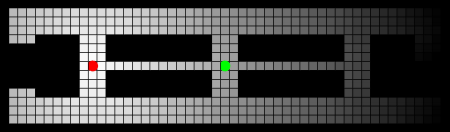
\includegraphics[scale=0.72]{images/autnmRobot_MDPValueFunction.png}
	\caption{Ein Beispiel einer Wertefunktion bei unendlichem Planungshorizont. Diese Wertefunktion induziert die Strategie in Abbildung \ref{autnmRobot_detA} (aus \cite{thrun2005probabilistic}).}
	\label{autnmRobot_policy}
\end{figure}

In dieser Ausarbeitung wurde der MDP mit endlicher Zustandsmenge definiert. Es gibt auch die Möglichkeit den MDP mit einer unendlichen Zustandsmenge zu definieren, was allerdings die Komplexität der Berechnung einer optimalen Strategie erhöht. 


\section{Ausblick}
\label{sec:pomdp}
\subsection{POMDP}
\begin{figure}[ht]
	\centering
	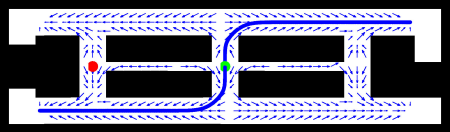
\includegraphics[scale=0.72]{images/autnmRobot_POMDPPathA.png}
	\caption{Die Strategie zu einem Zeitpunkt, an dem die Orientierung des Roboters noch nicht feststeht. Um zu vermeiden, auf Grund der Symmetrie der Umgebung in die falsche Richtung zu fahren ist es sinnvoll an den linken bzw. den rechten Rand der Umgebung zu fahren, die sich deutlich unterscheiden (aus \cite{thrun2005probabilistic}).}
	\label{autnmRobot_POMDPPathA}
\end{figure}

\begin{figure}[ht]
	\centering
	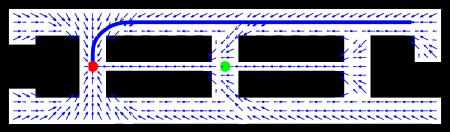
\includegraphics[scale=0.72]{images/autnmRobot_POMDPPathB.png}
	\caption{Die Strategie zu dem Zeitpunkt, an dem durch den Markanten Punkt am rechten Rand der Roboter den Ort des Zieles mit sehr hoher Wahrscheinlichkeit kennt (aus \cite{thrun2005probabilistic}).}
	\label{autnmRobot_POMDPPathB}
\end{figure}

\begin{figure}[ht]
	\centering
	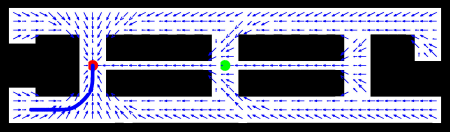
\includegraphics[scale=0.72]{images/autnmRobot_POMDPPathC.png}
	\caption{Die Strategie zu dem Zeitpunkt, an dem durch den Markanten Punkt am linken Rand der Roboter den Ort des Zieles mit sehr hoher Wahrscheinlichkeit kennt (aus \cite{thrun2005probabilistic}).}
	\label{autnmRobot_POMDPPathC}
\end{figure}

Bisher wurde angenommen, dass die Sensoren des Roboters jederzeit den exakten Zustand der Umgebung wahrnehmen können. In der Praxis liefern Sensoren allerdings lediglich ein verrauschtes Abbild der Umgebung. Daher kann der Zustand nur bis zu einem gewissen Grade geschätzt werden. Natürlich gibt es Bereiche der Umgebung, in denen Sensoren mehr oder weniger gut funktionieren.

Zur Veranschaulichung dieser Problematik wird wieder das in Kapitel \ref{sec:planning} erläuterte Beispiel verwendet. Das einzige Unterscheidungsmerkmal findet sich am linken bzw. rechten Ende der Umgebung. Direkt in Richtung eines möglichen Zielortes zu fahren würde eine 50\% Chance mit sich bringen das Ziel zu verpassen und stattdessen zu dem entsprechenden Ort auf der anderen Seite zu fahren. Optimalerweise muss der Roboter nun also zuerst in eine der Ecken fahren um sicher feststellen zu können, wo sich das genau Ziel befindet. (Das Ziel selbst ist für die Sensoren des Roboters nicht wahrnehmbar)

Bei der Roboterpfadplanung muss nun in Betracht gezogen werden, wann es sich lohnt erst mal höhere Kosten auf sich zu nehmen, um die Wahrscheinlichkeit zu erhöhen den richtigen Umgebungszustand zu schätzen. Außerdem können bestimmte Pfade mehr oder weniger attraktiv werden, je nach dem wie gut die Sensoren des Roboters auf ihnen funktionieren. So kann bei der Pfadplanung beispielsweise eine Zone in der Lokalisierung mit Hilfe von GPS nur schwer möglich ist, gemieden werden, falls es bessere Alternativen gibt.

Um diese Unsicherheit in der Wahrnehmung der Umgebung zu modellieren gibt es eine Erweiterung für den MDP. Das erweiterte Modell, der POMDP, sieht formal in erster Linie dem MDP sehr ähnlich. Es gibt eine Menge von Zuständen $S$, eine Menge von Aktionen $A$, ein Zustandsübergangsmodell $T$ sowie eine Gütefunktion $r$. Hinzu kommen
\begin{itemize}
	\item die Menge der Beobachtungen $Z = \{z_1, z_2, ..., z_{|Z|}\}$
	\item die Menge der Beobachtungswahrscheinlichkeiten $O(z_i, a, s_j)$
\end{itemize}
durch die ausgedrückt wird, wie wahrscheinlich es ist, dass bei Aktion $a$ in Zustand $s_j$ die Beobachtung $z_i$ gemacht wird.

\subsection{Strategien aus POMDP}
Um auf Basis des POMDP eine Strategie zu entwickeln betrachtet man häufig eine Wertefunktion $V(b)$ über die Wahrscheinlichkeitsverteilung über alle Zustände \cite{roy2005finding}. Diese Wahrscheinlichkeitsverteilung $b$ wird auch \emph{belief space} genannt. Statt den Zustand wie bei dem MDP immer sicher zu wissen verwenden wir jetzt also die Wahrscheinlichkeitsverteilung $b$, der für jeden Zustand die Wahrscheinlichkeit angibt, dass sich die Umgebung in diesem Zustand befindet. Diese Wahrscheinlichkeitsverteilung wird anhand der Beobachtungen $Z$ und den Beobachtungswahrscheinlichkeiten $O$ verändert.

Konkrete Algorithmen zur exakten und/oder approximativen Berechnung von Strategien finden sich in \cite{cassandra1995acting}, \cite{roy2005finding} und \cite{thrun2005probabilistic}.

%%%%%%%%%%%%%%%%%%%%%%%%%%%%%%%%%%%%%%%%%%%%%%%%%%%%%%%%%%%%%%%%%%%%%%%%%
% Literaturverzeichnis (in literatur.bib, z.B. mit Jabref editieren) 
\bibliographystyle{plain}
\bibliography{literatur}
\end{document}